%
% File: chap 2.tex
% Author: Abhimanyu Bambhniya
% Description: Literature review
%
\let\textcircled=\pgftextcircled
\chapter{Literature Review}
\label{chap:Literature_Review}

\section{Overview}
\paragraph{}

This chapter reviews many other works that have been done at various institutes and companies. In-memory computation being a great tool in modern day industries ,business customers, retailers and banks , to quickly detect patterns in real time, analyze massive data volumes on the fly, and perform their operations quickly.The drop in memory prices in the modern market is a major factor contributing to the increasing popularity of in-memory computing technology. This has also made in-memory computing economical among a wide variety of applications. Other major applications in industry
are:-
\begin{itemize}
\item Investment banking 
\item Insurance claim processing \& modeling 
\item Real-time ad platforms 
\item Real-time sentiment analysis 
\item Merchant platform for online games 
\item Hyper-local advertising 
\item Geo spatial/GIS processing 
\item Medical imaging processing 
\item Natural language processing \& cognitive computing 
\item Real-time machine learning 
\item Complex event processing of streaming sensor data 
\end{itemize}

\section{X-SRAM:Boolean Computation in 8T SRAM}
\paragraph{}

In-memory techniques tend to bypass the von-Neumann bottleneck by accomplishing computations inside the memory array. In other words, in-memory-compute blocks store data exactly like a standard memory, however, they enable additional operations without expensive area or energy overheads by adding peripherals .[2] discusses simple Boolean operation of NAND and NOR with traditional 8T SRAM cell.[2] also proposes Voltage divider scheme for 8T cell to perform XOR and IMP operation.

\section{Multi bit dot product engine}
\paragraph{}

In [3], it show that the standard 8T SRAM array can be configured as an analog-like in-memory multi-bit dot product engine. By applying appropriate analog voltages at the read-ports of the 8T SRAM array, and sensing the output current, an approximate analog-digital dot-product engine can be implemented. [3] present two different configurations for enabling multi-bit dot product computations in the 8T SRAM cell array, without modifying the standard bit-cell structure. 

\section{Machine-Learning Classifier in 6T SRAM}
\paragraph{}

\begin{figure}[h]
\centering
\begin{subfigure}{0.4\textwidth}
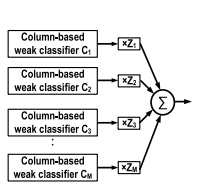
\includegraphics[width=1\linewidth]{EACB1.PNG} 
\caption{ Logical structure of a resulting strong classifier}
\label{fig:Figure}
\end{subfigure}

\begin{subfigure}{0.4\textwidth}
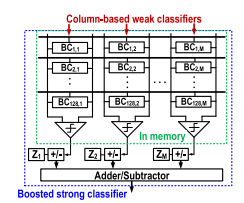
\includegraphics[width=1\linewidth]{EACB2.PNG}
\caption{ its implementation within the in-memory classifier architecture}
\label{fig:Figure}
\end{subfigure}
 
\caption{Illustration of EACB[4] }
\label{fig:Figure}
\end{figure}

In [4], it presents a machine-learning classifier in which computations are performed in a standard 6T SRAM, which stores the machine-learning model.The Peripheral circuits are implemented mixed-signal weak classifiers via the columns of the SRAM, and the training algorithm enables a strong enough classifier through boosting.[4] computes multi-input Multiply-and-Accumulate (MAC) but obtains a binary output for the weak-classifier in each column. Due to this limitation, it achieves a low accuracy of ~90\% for MNIST dataset.

\section{Pattern Recognition in SRAM}
\paragraph{}

In [5], 6T-SRAM cells have also been used to implement dot products in analog domain for pattern recognition.[5] was one of the earliest paper to present the concept of compute memory, where computation is deeply embedded into the SRAM. This deep embedding enables multi-row read access and analog signal processing. Compute memory exploits the relaxed precision and linearity requirements of pattern recognition applications. Bit-line computing in SRAMs has been used to implement custom accelerators: approximate dot products in analog domain for pattern recognition[5]. 
